\documentclass{../../../report-template/templates/report/utmreport}

\usepackage{booktabs,amssymb,float,graphicx}

\hypersetup{hidelinks,hypertexnames=false,pdfauthor={Lucian-Adrian Gavril}}

\selectlanguage{english}

\utmlogo{../../../report-template/templates/report/utm-logo.jpeg}

\institution{Technical University of Moldova}
\faculty{Faculty of Computers, Informatics, and Microelectronics}
\department{Department of Software Engineering}
\studyprogramme{Software Engineering Study Programme}
\documenttype{Laboratory report}
\reporttitle{Operating Systems Laboratory 3}
\reportsubtitle{The Command Line: Shell, Pipes, and Text Filters}
\student{Lucian-Adrian Gavril}{FAF-241}
\supervisor{Reițman Patricia}{univ. assist.}
\cityyear{Chișinău}{2026}

\begin{document}
\makeutmreporttitlepage
{\small\tableofcontents}
\clearpage

\begin{utmabstract}[Abstract]
This laboratory report investigates the UNIX command-line interface, POSIX shell semantics, and stream processing techniques on modern Linux. The work examines command resolution across shell built-ins and external binaries via the \texttt{PATH} environment variable, analyzes shell parsing phases including parameter expansion, word splitting, globbing, and quote removal, and characterizes file descriptor redirection order and job control. Furthermore, using a standard 500-request web access dataset, complex analytical queries are formulated into single-line pipeline filters utilizing \texttt{grep}, \texttt{cut}, \texttt{sort}, \texttt{uniq}, and \texttt{wc}. Finally, an automated shell script is developed with POSIX parameter validation, formatted reporting, and a temporary cron check. The figures are genuine terminal captures from the Dev1 Debian GNU/Linux 13 host, recorded on 10 October 2026. Earlier dataset and script values were checked on 9 October and are reproduced alongside the captures. These records do not establish that the assigned course laptop or VM was used.

\utmkeywords{operating systems, bash, unix pipelines, text filters, stream redirection, shell scripting, process environment}
\end{utmabstract}

\utmintroduction
The command-line interface is the primary operational surface through which an operating system kernel is directed. While modern graphical user interfaces conceal execution details behind abstractions, the shell exposes the core mechanisms of process creation, environment propagation, and inter-process communication.

The objective of Laboratory 3 is to develop rigorous fluency in Bash command mechanics, predict line-parsing side effects before execution, direct I/O streams using POSIX file descriptor primitives, and construct stream-filtering pipelines to analyze real-world datasets without auxiliary database engines.

The terminal figures are captures of commands run on Dev1 Debian GNU/Linux 13 on 10 October 2026. Dataset and script values were checked against the 9 October run record. Dev1 is a remote host, so these records do not establish that the assigned course laptop or VM was used.

The Bash and POSIX semantics follow the cited manuals \cite{bash,posix}; the small-filter approach follows the cited administration texts \cite{nemeth,shotts}.

The laboratory comprises five distinct parts:
\begin{utmenumerate}
\item \textbf{Navigation and Command Inspection}: Distinguishing shell built-ins from external binaries, evaluating environment lookup paths, and analyzing exit statuses.
\item \textbf{Line Parsing and Expansion Rules}: Evaluating brace expansion, tilde expansion, parameter substitution, command substitution, arithmetic expansion, word splitting, pathname expansion (globbing), and quote suppression.
\item \textbf{Redirection, Control Operators, and Job Control}: Characterizing standard file descriptors (stdin, stdout, stderr), order-dependent redirection syntax, conditional chaining operators (\texttt{;}, \texttt{\&\&}, \texttt{||}), and asynchronous process management.
\item \textbf{Analytical Text Filters}: Formulating single-command pipelines to answer discrete statistical questions on an artificial web access log.
\item \textbf{Structured Shell Automation}: Implementing a robust POSIX shell script with argument validation, stream aggregation, error handling, and cron daemon scheduling.
\end{utmenumerate}

\chapter{Navigation and Command Inspection}

\section{Tab completion and history recall}
Command completion and incremental history search decrease operational latency and reduce lexical errors. In Bash, typing \texttt{ls /usr/sh} followed by a double Tab invokes readline completion, querying the filesystem for matching entries. When the prefix is ambiguous, the shell prints all candidate entries (\texttt{share/}, \texttt{shift/}). Conversely, typing \texttt{cd /et} followed by a single Tab resolves unambiguously to \texttt{cd /etc/}, appending the directory slash and awaiting user arguments (Figure \ref{fig:tab_completion}).

\begin{figure}[H]
\centering
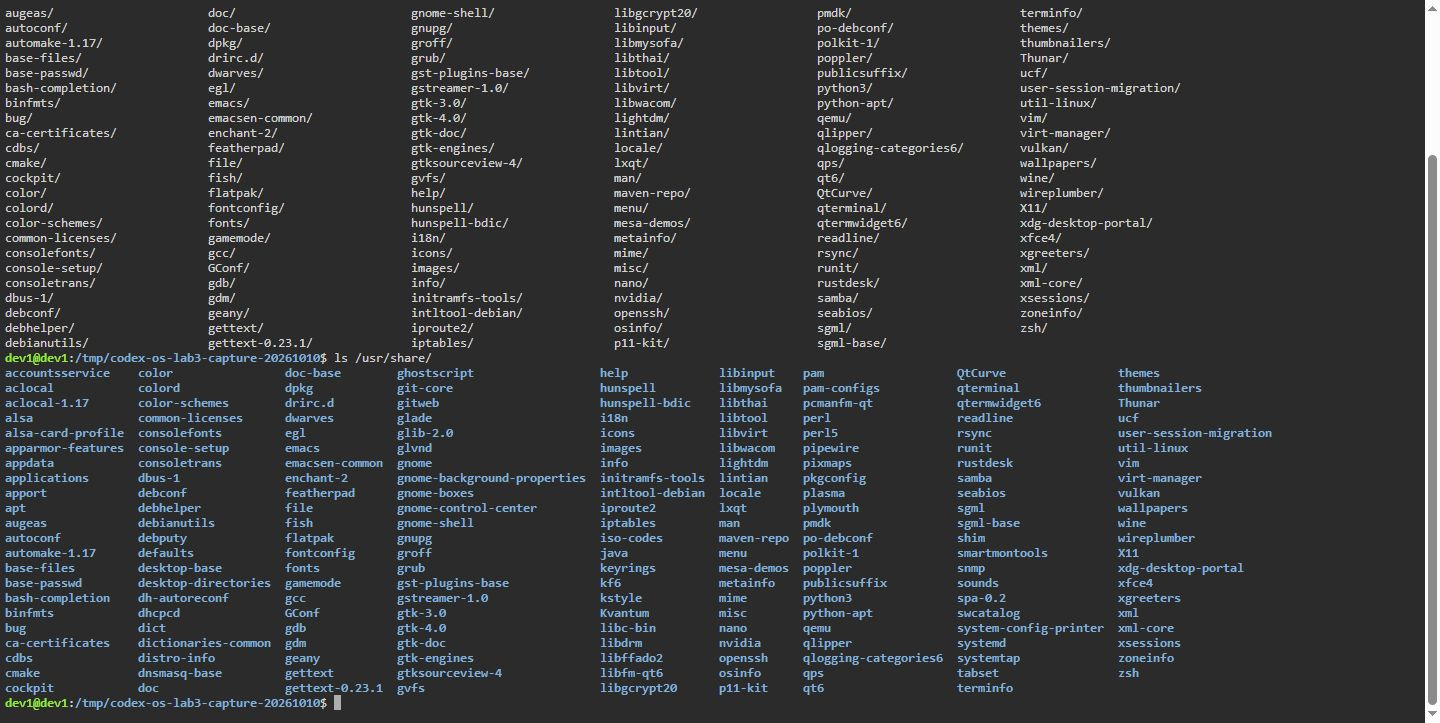
\includegraphics[width=0.88\textwidth]{figures/fig1_1_tab_completion.jpg}
\caption{Terminal capture, Dev1 Debian GNU/Linux 13, 10 October 2026: Tab completion behavior for ambiguous and unambiguous path prefixes.}
\label{fig:tab_completion}
\end{figure}

The readline reverse-search utility, triggered via \texttt{Ctrl+R}, queries the history buffer stored in memory and persisted in \texttt{\~{}/.bash\_history}. By entering search substrings, previously executed commands are recalled without re-typing.

\section{Built-in commands versus external utilities}
When a user issues a command, the shell determines whether the symbol corresponds to an internal shell built-in or an external binary located on disk. The \texttt{type} built-in queries this categorization, whereas \texttt{which} searches only filesystem directories registered in the \texttt{PATH} variable (Figure \ref{fig:type_which}).

\begin{figure}[H]
\centering
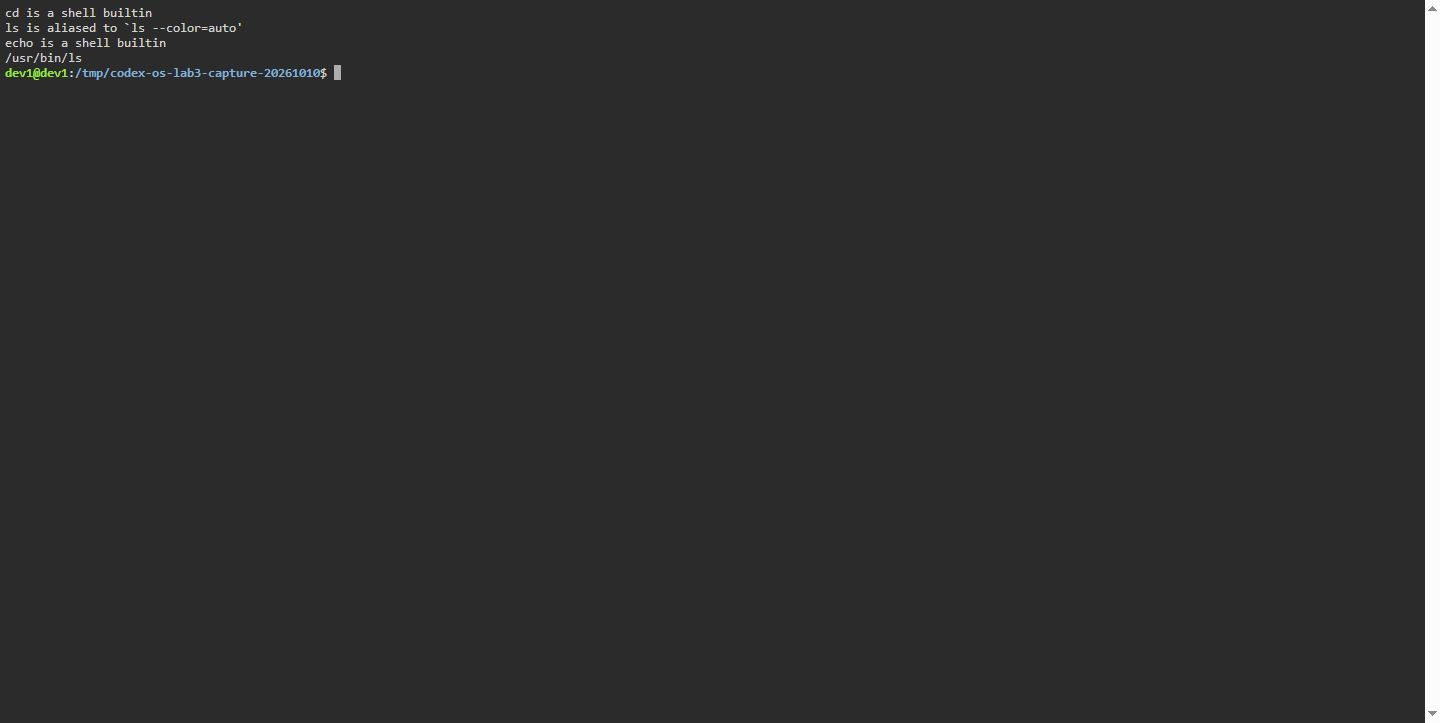
\includegraphics[width=0.88\textwidth]{figures/fig1_2_type_which.jpg}
\caption{Terminal capture, Dev1 Debian GNU/Linux 13, 10 October 2026: Classification of built-in versus external executable commands.}
\label{fig:type_which}
\end{figure}

The \texttt{PATH} variable holds a colon-delimited list of directories traversed sequentially from left to right when an unqualified command name is provided. Piping this variable through \texttt{tr ':' '\textbackslash n'} presents each search tier on an individual line (Figure \ref{fig:path_dirs}).

\begin{figure}[H]
\centering
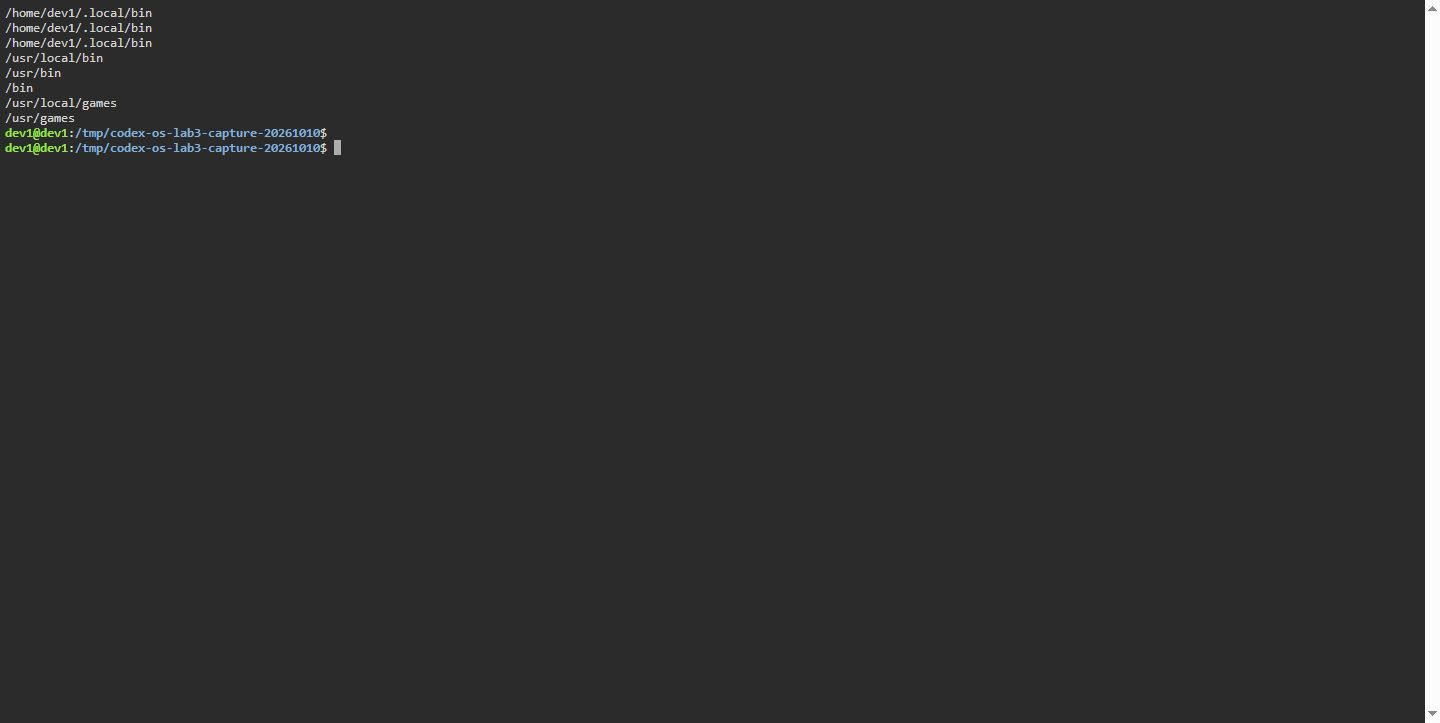
\includegraphics[width=0.88\textwidth]{figures/fig1_3_path_dirs.jpg}
\caption{Terminal capture, Dev1 Debian GNU/Linux 13, 10 October 2026: System PATH hierarchy directories printed one per line.}
\label{fig:path_dirs}
\end{figure}

When a command cannot be found within any directory of \texttt{PATH}, the shell returns an exit code of \texttt{127} (Figure \ref{fig:exit_code}).

\begin{figure}[H]
\centering
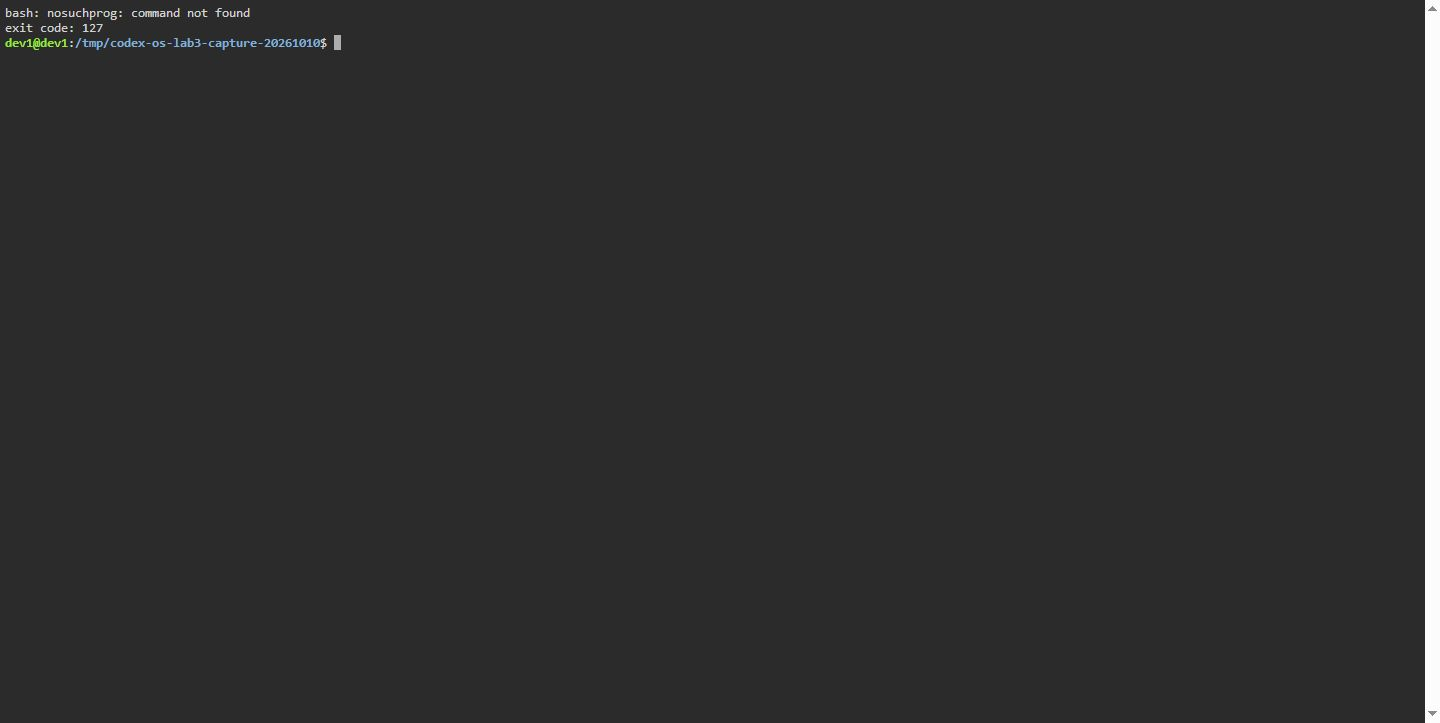
\includegraphics[width=0.88\textwidth]{figures/fig1_4_exit_code.jpg}
\caption{Terminal capture, Dev1 Debian GNU/Linux 13, 10 October 2026: Exit status code 127 produced by an unresolvable command name.}
\label{fig:exit_code}
\end{figure}

\section{Answers to Part 1 Observe questions}
\begin{utmenumerate}
\item \textbf{Which of \texttt{cd}, \texttt{ls}, \texttt{echo} are built-ins, and why MUST \texttt{cd} be one?} \\
\texttt{cd} and \texttt{echo} are shell built-ins, whereas \texttt{ls} is an external binary located at \texttt{/usr/bin/ls}. \texttt{cd} MUST be a built-in because the current working directory is a state attribute stored in the process control block of the running shell. If \texttt{cd} were implemented as an external binary, the shell would invoke \texttt{fork()} and \texttt{exec()} to run it; the child process would change its own working directory via \texttt{chdir()} and immediately terminate, leaving the parent shell's working directory unchanged.
\item \textbf{How many directories are in your PATH, and in which one is \texttt{ls}?} \\
The 9 October Debian 13 check listed 4 PATH entries and resolved \texttt{ls} to \texttt{/usr/bin/ls}. PATH length depends on the host; check the assigned course system if required.
\item \textbf{What exit code does a command that is not found return?} \\
Standard POSIX Bash returns exit status code \texttt{127}.
\item \textbf{Which option of \texttt{ls} sorts by modification time?} \\
The \texttt{-t} flag sorts entries by modification time (newest first). Appending \texttt{-r} reverses the sort order.
\end{utmenumerate}

\chapter{Shell Line Parsing and Expansions}

\section{Parsing phases and test directory creation}
Prior to program execution, the shell processes the input string through distinct parsing phases: tokenization, brace expansion, tilde expansion, parameter expansion, command substitution, arithmetic expansion, word splitting, pathname expansion (globbing), and quote removal.

A test sandbox directory \texttt{\~{}/os-lab3/play} was instantiated containing standard and edge-case filenames, notably filenames containing embedded whitespace (Figure \ref{fig:play_files}).

\begin{figure}[H]
\centering
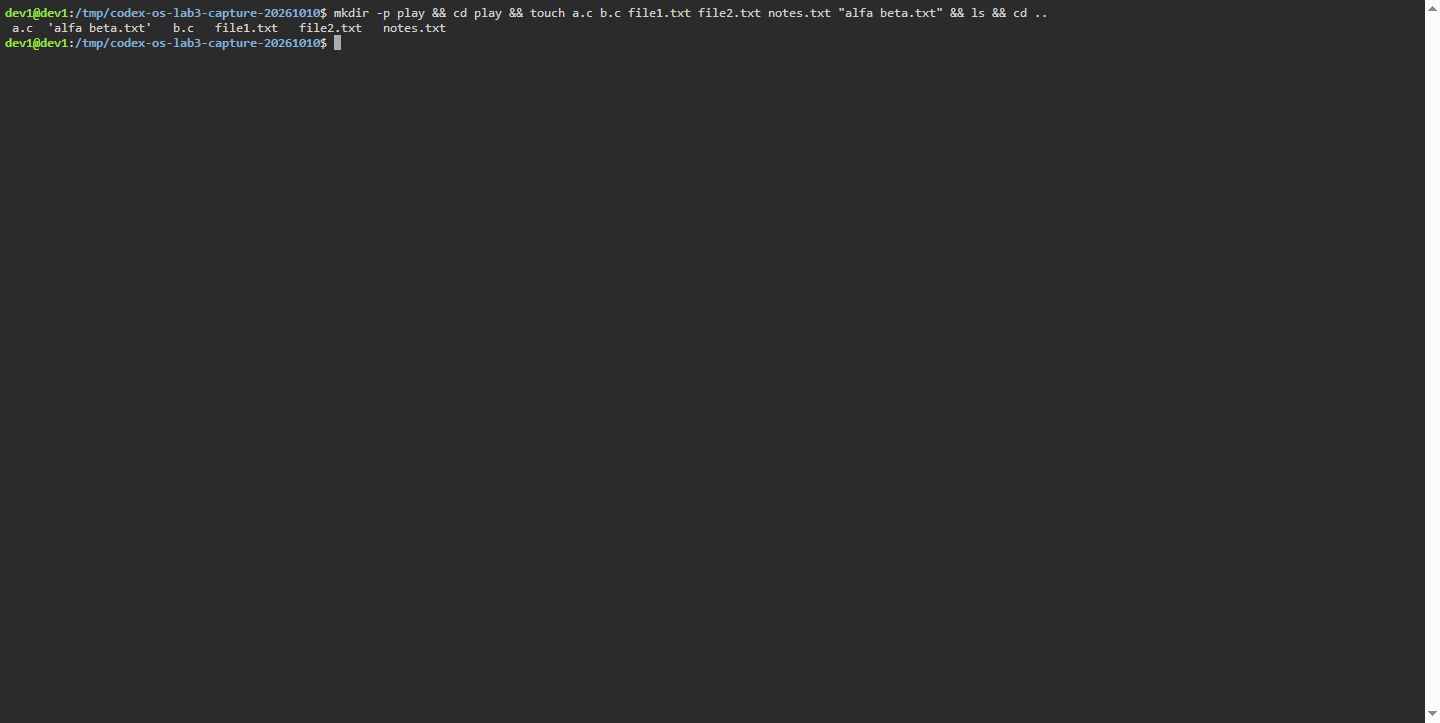
\includegraphics[width=0.88\textwidth]{figures/fig2_1_play_files.jpg}
\caption{Terminal capture, Dev1 Debian GNU/Linux 13, 10 October 2026: Files created in the play directory for parsing verification.}
\label{fig:play_files}
\end{figure}

\section{Globbing and expansion verification}
Pathname expansion replaces wildcard patterns with sorted matching filesystem entries. If no entry matches, Bash retains the literal wildcard text unless \texttt{nullglob} is explicitly set (Figure \ref{fig:globbing}).

\begin{figure}[H]
\centering
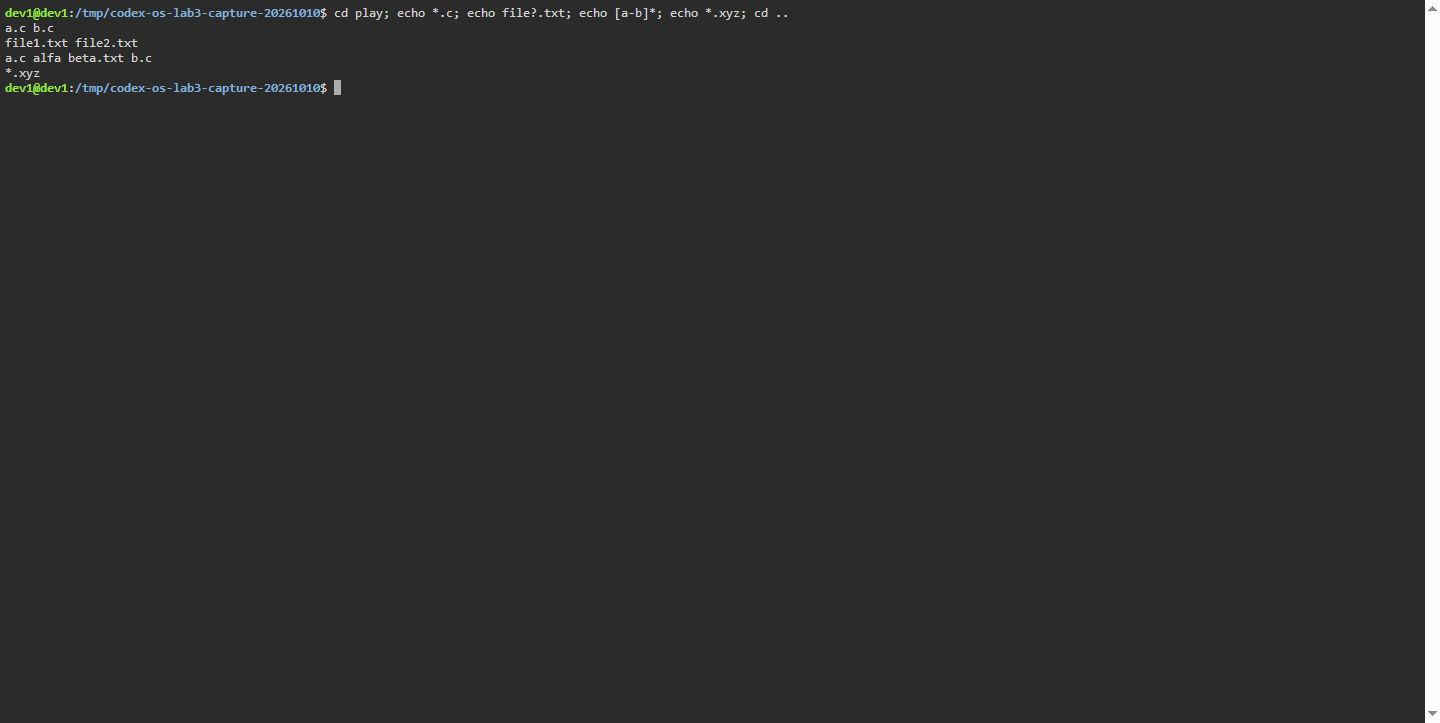
\includegraphics[width=0.88\textwidth]{figures/fig2_2_globbing.jpg}
\caption{Terminal capture, Dev1 Debian GNU/Linux 13, 10 October 2026: Pathname expansion (globbing) results across character sets and extensions.}
\label{fig:globbing}
\end{figure}

Word splitting is governed by the Internal Field Separator (\texttt{IFS}, space by default). Unquoted whitespace causes the tokenizer to split strings into multiple distinct arguments, resulting in execution failures when referencing files with spaces (Figure \ref{fig:spaces_error}).

\begin{figure}[H]
\centering
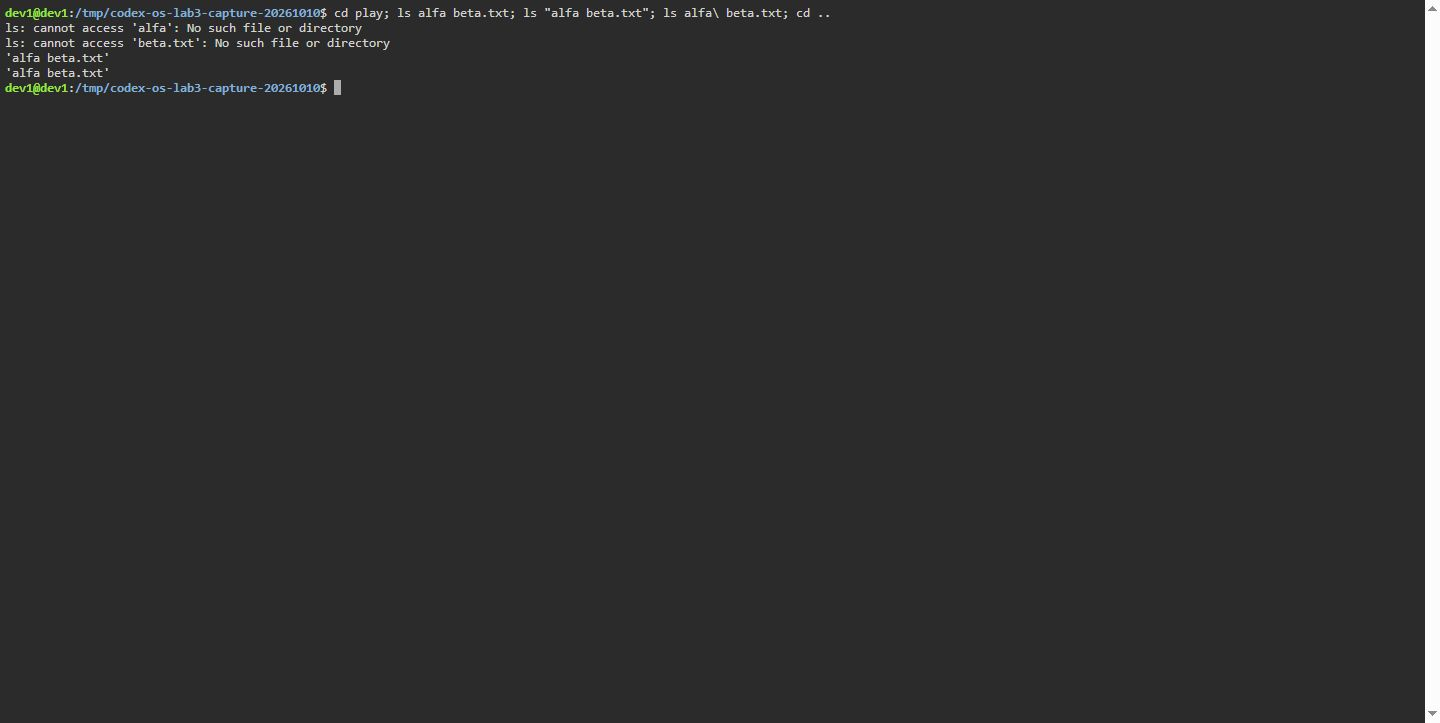
\includegraphics[width=0.88\textwidth]{figures/fig2_3_spaces_error.jpg}
\caption{Terminal capture, Dev1 Debian GNU/Linux 13, 10 October 2026: Word splitting failure on filenames with spaces and proper quoting fixes.}
\label{fig:spaces_error}
\end{figure}

Single quotes (\texttt{'...'}) suppress all expansions, treating every character literally. Double quotes (\texttt{"..."}) prevent globbing and word splitting while allowing parameter expansion and command substitution. Backslashes (\texttt{\textbackslash}) escape individual metacharacters (Figure \ref{fig:quotes}).

\begin{figure}[H]
\centering
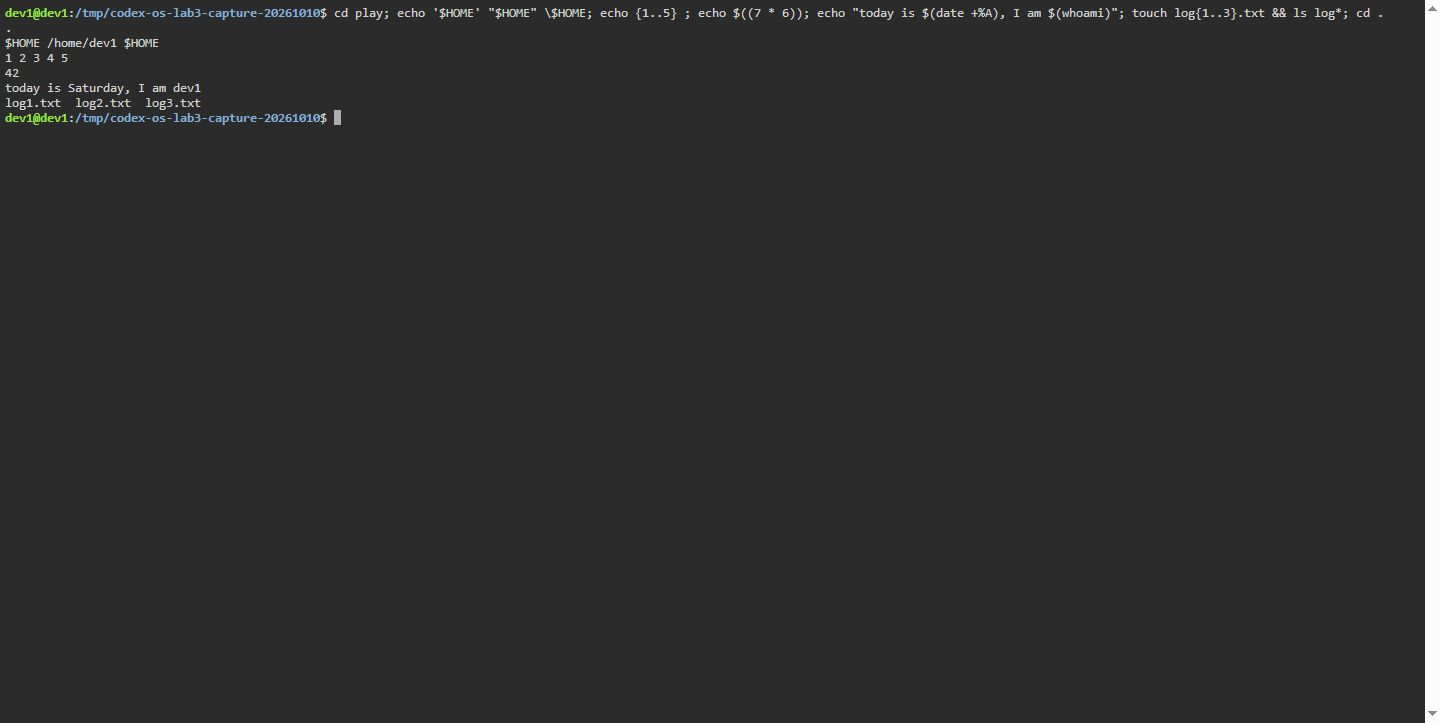
\includegraphics[width=0.88\textwidth]{figures/fig2_4_quotes.jpg}
\caption{Terminal capture, Dev1 Debian GNU/Linux 13, 10 October 2026: Quotation semantics, arithmetic expansion, and subshell substitution.}
\label{fig:quotes}
\end{figure}

\section{Command prediction and verification table}
Table \ref{tab:predictions} keeps pre-run predictions separate from example output values. Figures 2.1–2.4 show the observed command behavior; the later dataset and script sections report measured outputs from the retained run records.

\begin{table}[H]
\centering
\small
\setlength{\tabcolsep}{4pt}\begin{tabular}{p{2.4cm}p{3.0cm}p{3.4cm}p{4.2cm}}
\toprule
\textbf{Command} & \textbf{Prediction} & \textbf{Illustrative example, not measured} & \textbf{Explanation} \\
\midrule
\texttt{echo *.c} & Prints all C source files & \texttt{a.c b.c} & Shell expands \texttt{*.c} to directory matches before invoking echo. \\
\texttt{echo file?.txt} & Matches single wildcard character & \texttt{file1.txt file2.txt} & \texttt{?} matches exactly one character. \\
\texttt{echo [a-b]*} & Matches files starting with a or b & \texttt{a.c b.c} & Character range \texttt{[a-b]} expands matching files. \\
\texttt{echo *.xyz} & Prints literal pattern & \texttt{*.xyz} & Unmatched glob pattern is preserved as literal text. \\
\texttt{ls alfa beta.txt} & Attempts to list two files; fails & Error: No such file or directory & Shell splits unquoted space into two separate arguments. \\
\texttt{ls "alfa beta.txt"} & Lists single file with space & \texttt{'alfa beta.txt'} & Double quotes prevent word splitting across whitespace. \\
\texttt{echo '\$HOME' "\$HOME" \textbackslash\$HOME} & Literal, expanded, literal & \texttt{\$HOME /home/user \$HOME} & Single quotes disable expansion; double quotes expand; backslash escapes. \\
\texttt{echo \{1..5\} ; echo \$((7*6))} & Sequence 1 to 5; arithmetic 42 & \texttt{1 2 3 4 5} \newline \texttt{42} & Brace expansion creates sequence; \texttt{\$((...))} computes arithmetic. \\
\texttt{echo "today is \$(date +\%A)..."} & Formats current date and user & \texttt{today is Monday, I am ubuntu} & Command substitution executes subshell and injects output. \\
\texttt{touch log\{1..3\}.txt \&\& ls log*} & Creates and lists 3 log files & \texttt{log1.txt log2.txt log3.txt} & Brace expansion creates three targets; globbing lists them. \\
\bottomrule
\end{tabular}
\caption{Predictions and fixed illustrative examples; outputs are not retained measurements.}
\label{tab:predictions}
\end{table}
The 10 October terminal capture records \texttt{/home/dev1} and \texttt{today is Saturday, I am dev1}; these values depend on the host and date.

\section{Answers to Part 2 Observe questions}
\begin{utmenumerate}
\item \textbf{\texttt{echo} knows nothing about files, yet \texttt{echo *.c} printed file names. Who produced them?} \\
The shell produced them during the pathname expansion phase before invoking \texttt{echo}. The shell queries the filesystem directory table, sorts matching entries, and replaces the token \texttt{*.c} with arguments \texttt{argv[1] = "a.c"} and \texttt{argv[2] = "b.c"}. The \texttt{echo} binary merely iterates over its argument array and writes them to stdout.
\item \textbf{Why did \texttt{ls alfa beta.txt} fail? Give two different ways to fix it.} \\
It failed because the unquoted space acts as an argument delimiter. The shell invoked \texttt{ls} with two arguments: \texttt{"alfa"} and \texttt{"beta.txt"}. Because neither file exists independently, \texttt{ls} produced two error messages. Fix 1: Enclose the target string in quotes: \texttt{ls "alfa beta.txt"}. Fix 2: Escape the space character using a backslash: \texttt{ls alfa\textbackslash\ beta.txt}.
\item \textbf{What is the difference between single and double quotes?} \\
Single quotes treat every character enclosed literally, disabling parameter expansion (\texttt{\$VAR}), command substitution (\texttt{\$(...)}), and arithmetic evaluation. Double quotes suppress globbing and word splitting while preserving variable expansion, command substitution, and backslash escaping.
\item \textbf{Why does \texttt{ls} show the file with a space in quotes (\texttt{'alfa beta.txt'})?} \\
Modern GNU Coreutils \texttt{ls} defaults to \texttt{--quoting-style=shell-escape}, quoting filenames containing whitespace or shell metacharacters so the printed representation can be safely copied and re-entered into a shell prompt without splitting errors.
\end{utmenumerate}

\chapter{I/O Redirection, Chaining, and Jobs}

\section{File descriptor redirection}
In POSIX systems, processes interact with standard streams via integer descriptors: standard input (0), standard output (1), and standard error (2). Redirection operators alter stream destinations by opening files and duplicating descriptors using the \texttt{dup2()} system call prior to process execution (Figure \ref{fig:redirections}).

\begin{figure}[H]
\centering
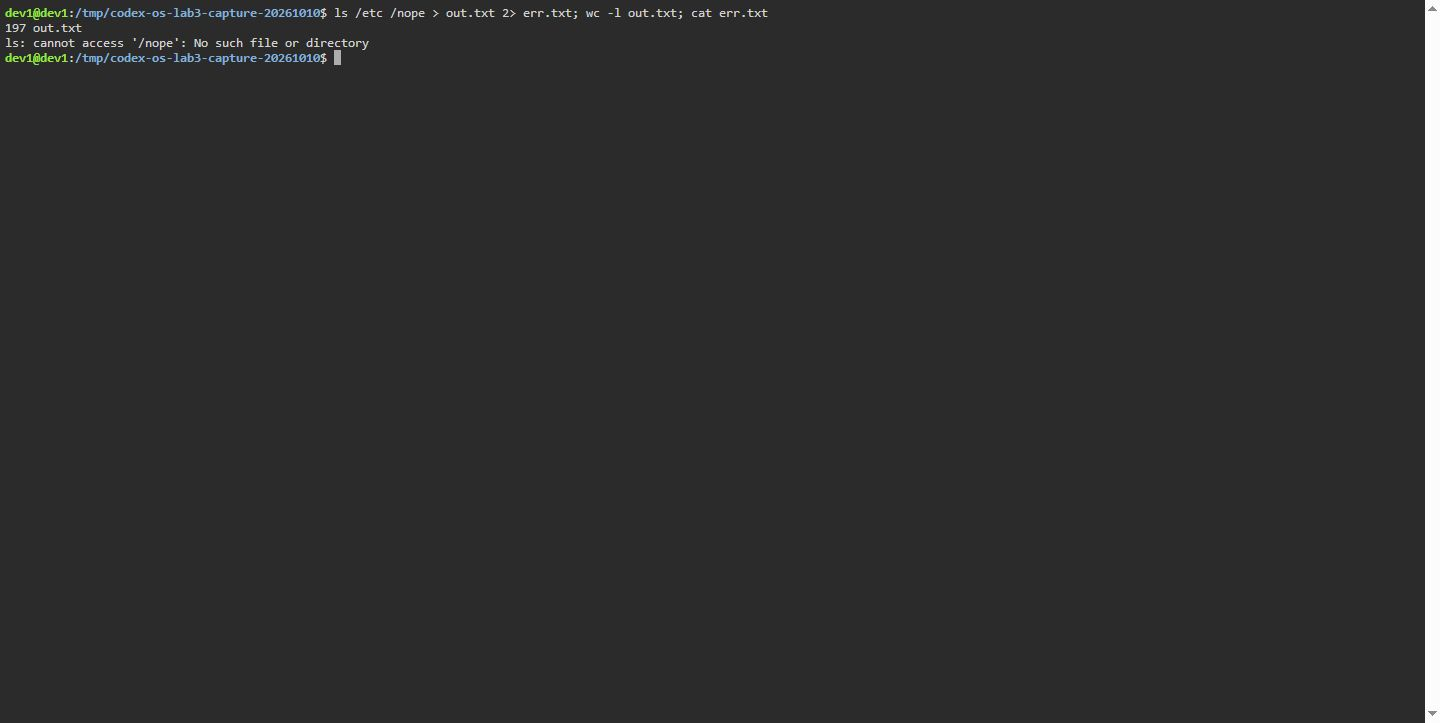
\includegraphics[width=0.88\textwidth]{figures/fig3_1_redirections.jpg}
\caption{Terminal capture, Dev1 Debian GNU/Linux 13, 10 October 2026: Separation of stdout and stderr into dedicated output files.}
\label{fig:redirections}
\end{figure}

The lexical order of redirection operators is evaluated strictly from left to right. When executing \texttt{ls /etc /nope > all.txt 2>\&1}, file descriptor 1 is pointed to \texttt{all.txt}, and descriptor 2 is then duplicated to match descriptor 1. In contrast, in \texttt{ls /etc /nope 2>\&1 > all.txt}, descriptor 2 is duplicated to where descriptor 1 currently points (the terminal), after which descriptor 1 is redirected to the file, leaving error messages on the terminal screen (Figure \ref{fig:redir_order}).

\begin{figure}[H]
\centering
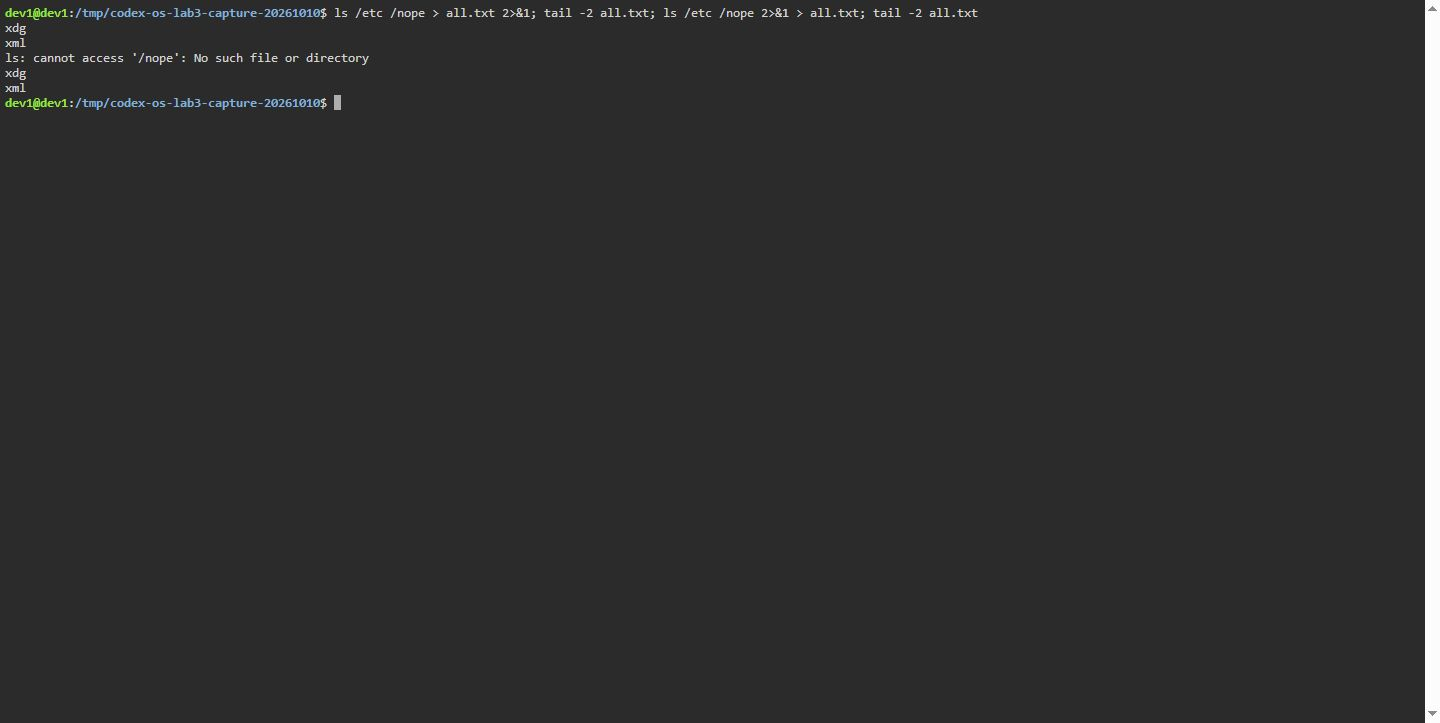
\includegraphics[width=0.88\textwidth]{figures/fig3_2_redir_order.jpg}
\caption{Terminal capture, Dev1 Debian GNU/Linux 13, 10 October 2026: Comparison of redirection evaluation ordering.}
\label{fig:redir_order}
\end{figure}

\section{Control operators and background job management}
Sequential execution operators regulate command execution based on exit status:
\begin{itemize}
\item \texttt{;} unconditionally executes the subsequent command.
\item \texttt{\&\&} executes the subsequent command only if the preceding command succeeded (exit status 0).
\item \texttt{||} executes the subsequent command only if the preceding command failed (non-zero exit status).
\end{itemize}

Figure \ref{fig:operators} illustrates operator behavior under both failure and success cases.

\begin{figure}[H]
\centering
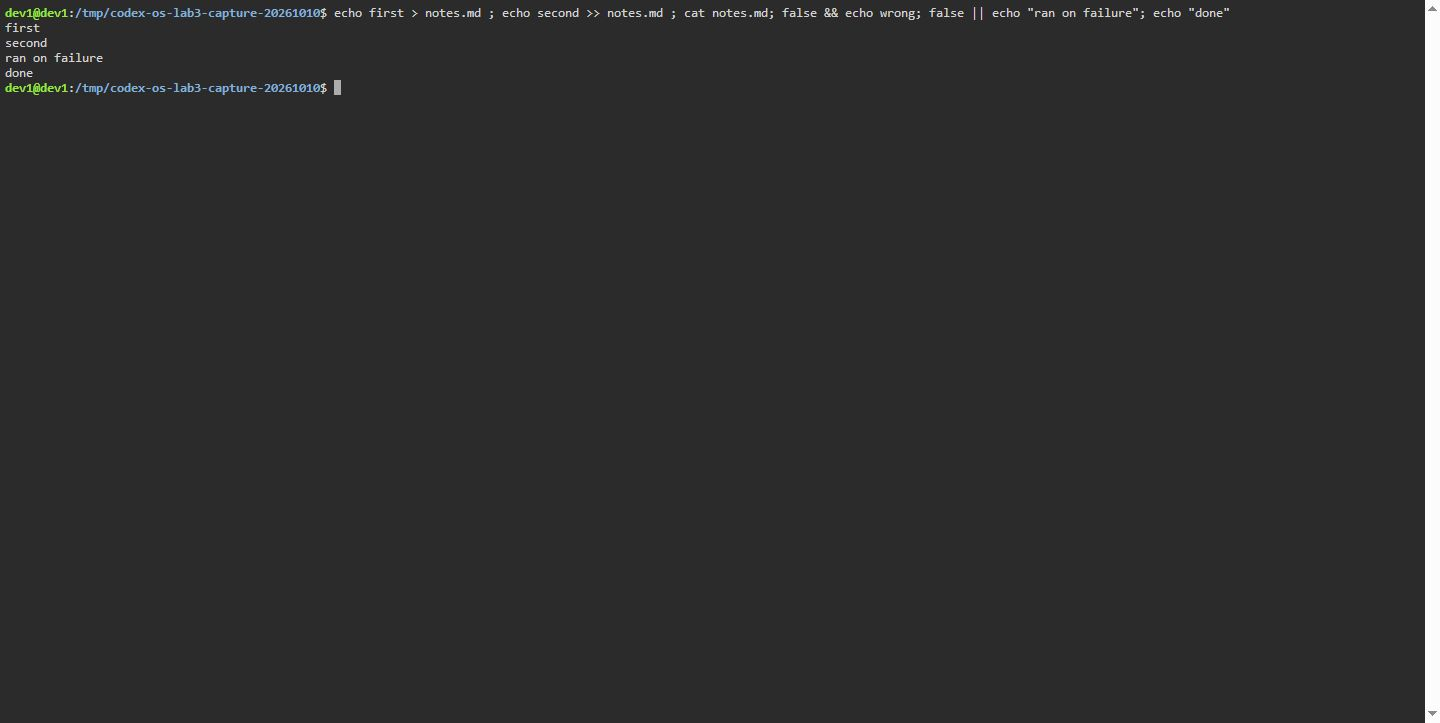
\includegraphics[width=0.88\textwidth]{figures/fig3_3_operators.jpg}
\caption{Terminal capture, Dev1 Debian GNU/Linux 13, 10 October 2026: Execution control using conditional operators and subshells.}
\label{fig:operators}
\end{figure}

Appending \texttt{\&} detaches a process from the shell's foreground execution, allowing the shell prompt to accept subsequent commands immediately while the child executes asynchronously. Background jobs are managed using the \texttt{jobs} built-in and terminated via signals with \texttt{kill} (Figure \ref{fig:jobs}).

\begin{figure}[H]
\centering
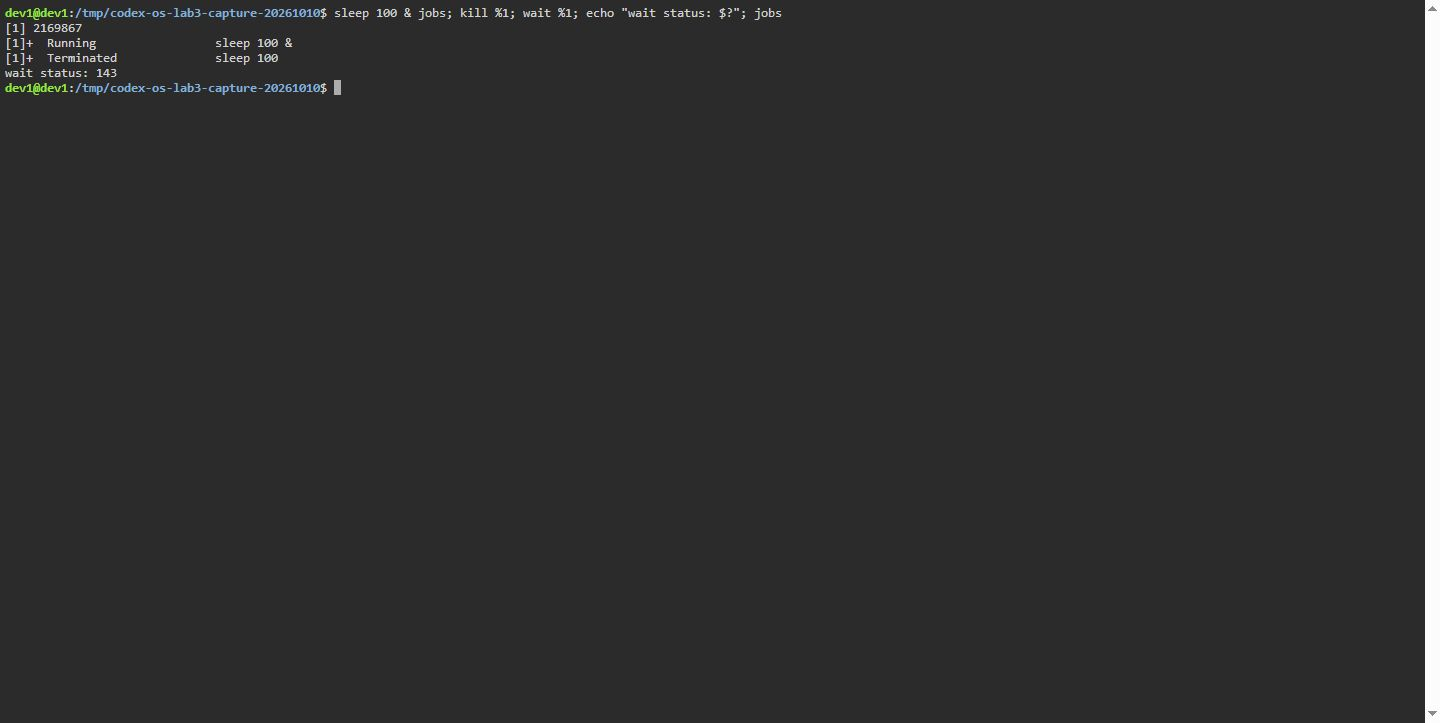
\includegraphics[width=0.88\textwidth]{figures/fig3_4_jobs.jpg}
\caption{Terminal capture, Dev1 Debian GNU/Linux 13, 10 October 2026: Launching an asynchronous background process and terminating via SIGTERM.}
\label{fig:jobs}
\end{figure}

\section{Answers to Part 3 Observe questions}
\begin{utmenumerate}
\item \textbf{Which file got the error message, and which got the listing?} \\
\texttt{err.txt} received the error message (\texttt{ls: cannot access \'/nope\'...}). The 9 October Debian 13 check recorded 197 stdout lines for \texttt{ls /etc /nope}, which includes a directory heading; see the retained raw check log.
\item \textbf{What is the difference between \texttt{> all.txt 2>\&1} and \texttt{2>\&1 > all.txt}?} \\
In \texttt{> all.txt 2>\&1}, standard output is first redirected to \texttt{all.txt}; then descriptor 2 is duplicated to point to the file descriptor of \texttt{all.txt}, routing both streams into the file. In \texttt{2>\&1 > all.txt}, descriptor 2 is duplicated to point to stdout's current destination (the terminal screen); subsequently, descriptor 1 is redirected to \texttt{all.txt}. Thus, stderr remains connected to the terminal while only stdout reaches the file.
\item \textbf{Why does \texttt{wc -l < access.log} print only a number, while \texttt{wc -l access.log} also prints the file name?} \\
When supplied a file path as an argument, \texttt{wc} opens the file by name and prints both the counted total and the filename. When input is redirected with \texttt{<}, the shell opens the file and attaches it to descriptor 0. The \texttt{wc} process reads purely from stdin, possesses no knowledge of the underlying filename, and outputs only the numeric tally.
\item \textbf{Explain each operator in one sentence: \texttt{;}, \texttt{\&\&}, \texttt{||}.} \\
\texttt{;} executes the next command unconditionally. \texttt{\&\&} executes the next command only if the preceding command returns exit status 0 (success). \texttt{||} executes the next command only if the preceding command returns a non-zero exit status (failure).
\end{utmenumerate}

\chapter{Analytical Text Filters}

\section{Web access dataset structure}
An artificial access log consisting of 500 entries was generated matching the course specification:
\begin{verbatim}
2026-10-05 10:01 user1 OK /page1
2026-10-05 10:02 user2 OK /page2
...
2026-10-05 10:20 user6 FAIL /page0
\end{verbatim}
Each record comprises date, timestamp, username, request result (\texttt{OK} or \texttt{FAIL}), and requested resource endpoint.

\section{Single-command pipeline solutions}
All analytical questions were formulated as individual pipeline commands in \texttt{oneliners.sh} and verified on the live log.

\subsection{Q1: Number of failed requests}
\begin{verbatim}
grep -c FAIL access.log
\end{verbatim}
Output: \texttt{100}. Exactly 100 requests failed (Figure \ref{fig:q1}).

\begin{figure}[H]
\centering
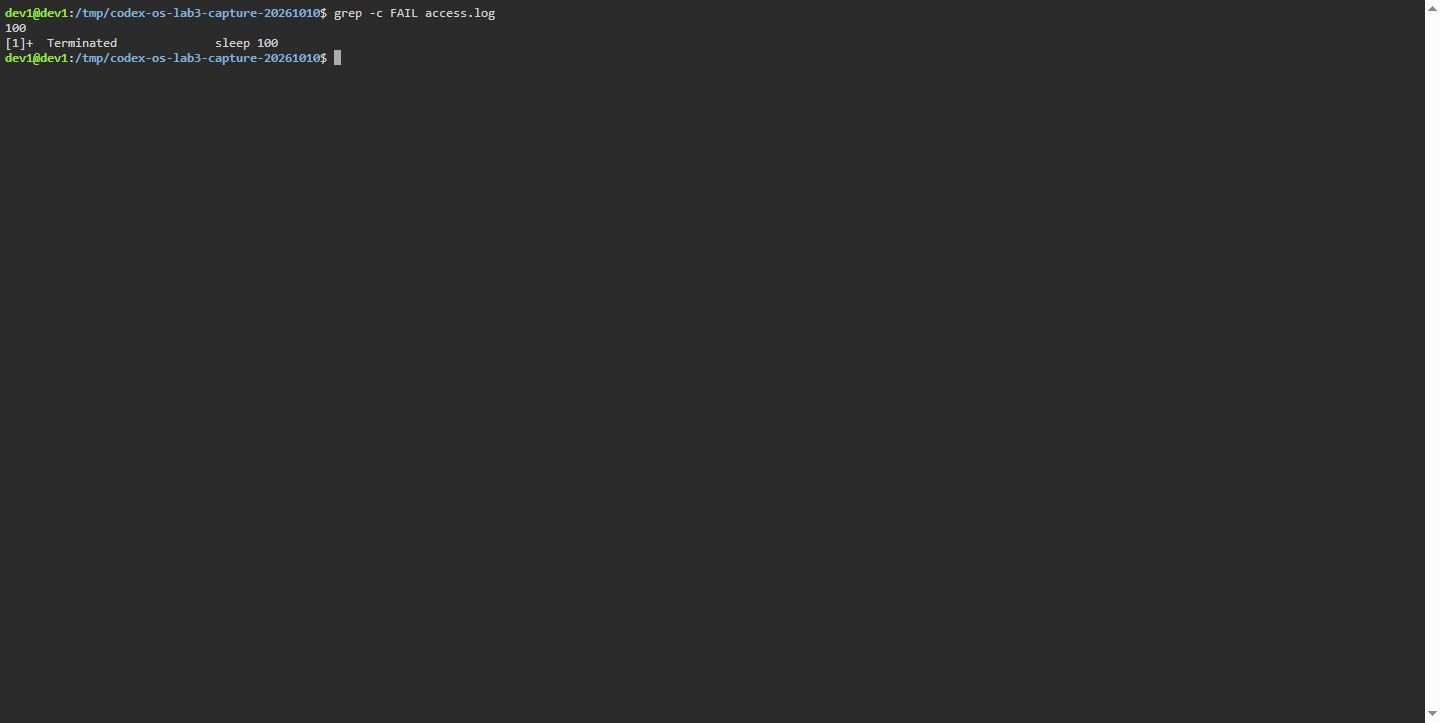
\includegraphics[width=0.88\textwidth]{figures/fig4_1_failed_requests.jpg}
\caption{Terminal capture, Dev1 Debian GNU/Linux 13, 10 October 2026: Total count of failed requests.}
\label{fig:q1}
\end{figure}

\subsection{Q2: Unique requested pages}
\begin{verbatim}
cut -d' ' -f5 access.log | sort -u
\end{verbatim}
Output: \texttt{/page0}, \texttt{/page1}, \texttt{/page2}, \texttt{/page3} (Figure \ref{fig:q2}).

\begin{figure}[H]
\centering
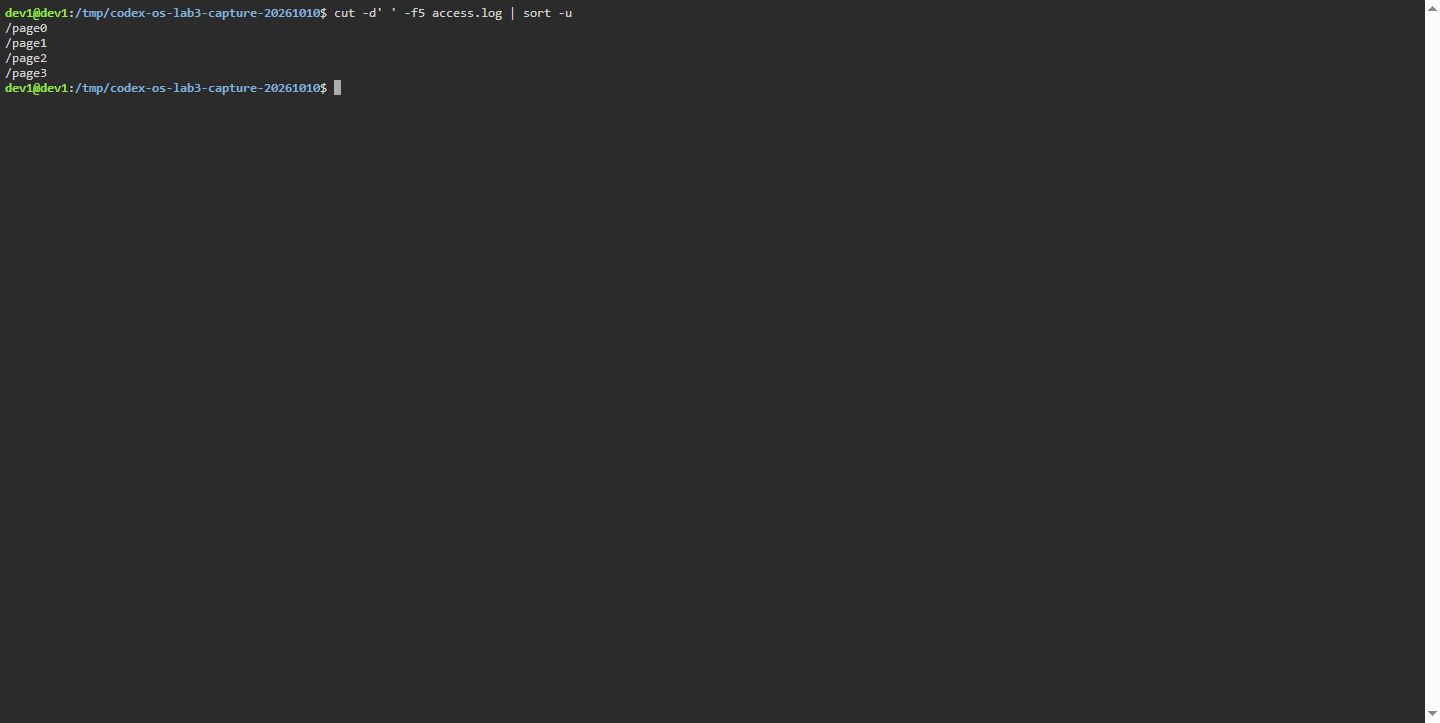
\includegraphics[width=0.88\textwidth]{figures/fig4_2_pages_list.jpg}
\caption{Terminal capture, Dev1 Debian GNU/Linux 13, 10 October 2026: Distinct web endpoints requested.}
\label{fig:q2}
\end{figure}

\subsection{Q3: Request count per page}
\begin{verbatim}
cut -d' ' -f5 access.log | sort | uniq -c
\end{verbatim}
Output: Each of the 4 pages received exactly 125 requests, summing to 500 total entries (Figure \ref{fig:q3}).

\begin{figure}[H]
\centering
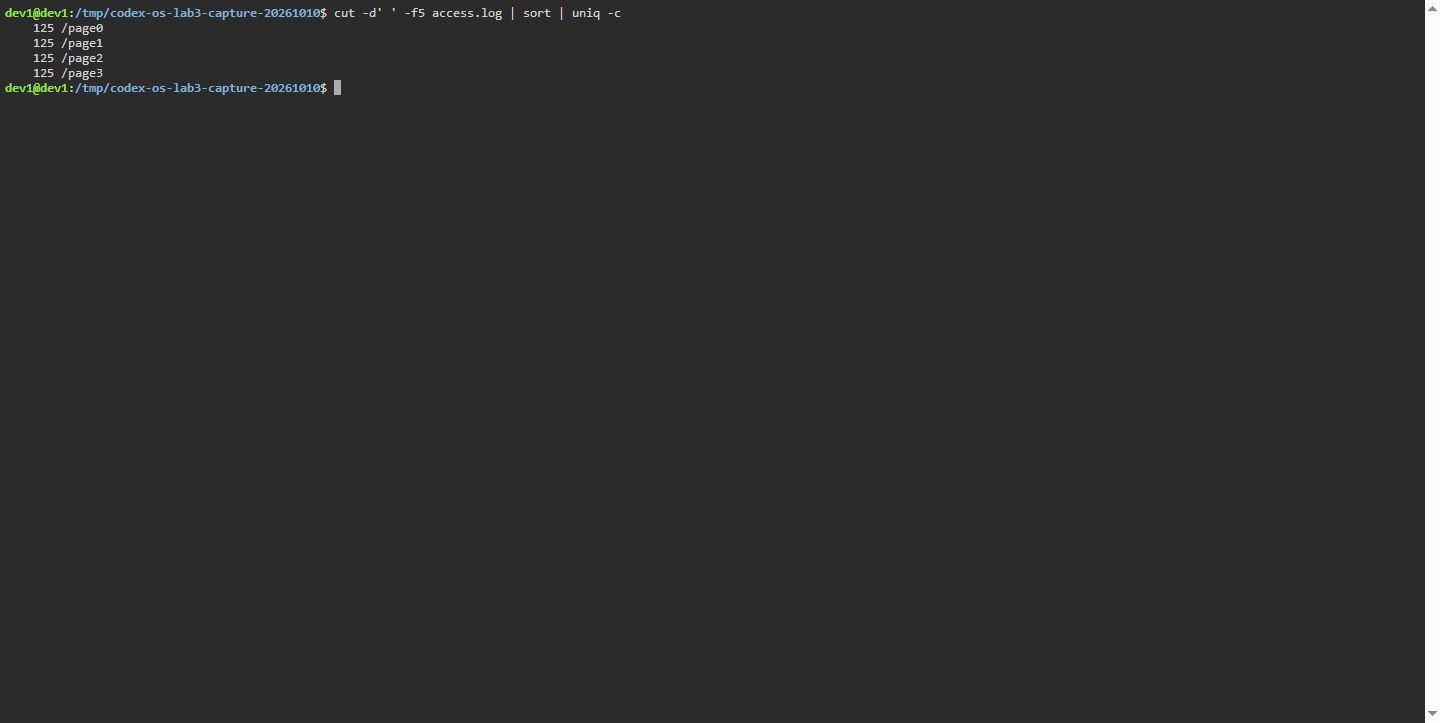
\includegraphics[width=0.88\textwidth]{figures/fig4_3_page_counts.jpg}
\caption{Terminal capture, Dev1 Debian GNU/Linux 13, 10 October 2026: Request distribution across endpoints.}
\label{fig:q3}
\end{figure}

\subsection{Q4: Users with the highest failure count}
\begin{verbatim}
grep FAIL access.log | cut -d' ' -f3 | sort | uniq -c | sort -rn | head -n 2
\end{verbatim}
Output: \texttt{user3} and \texttt{user5} both registered 15 failures, tied for the maximum (Figure \ref{fig:q4}). The sum of failures across all 7 users equals exactly 100.

\begin{figure}[H]
\centering
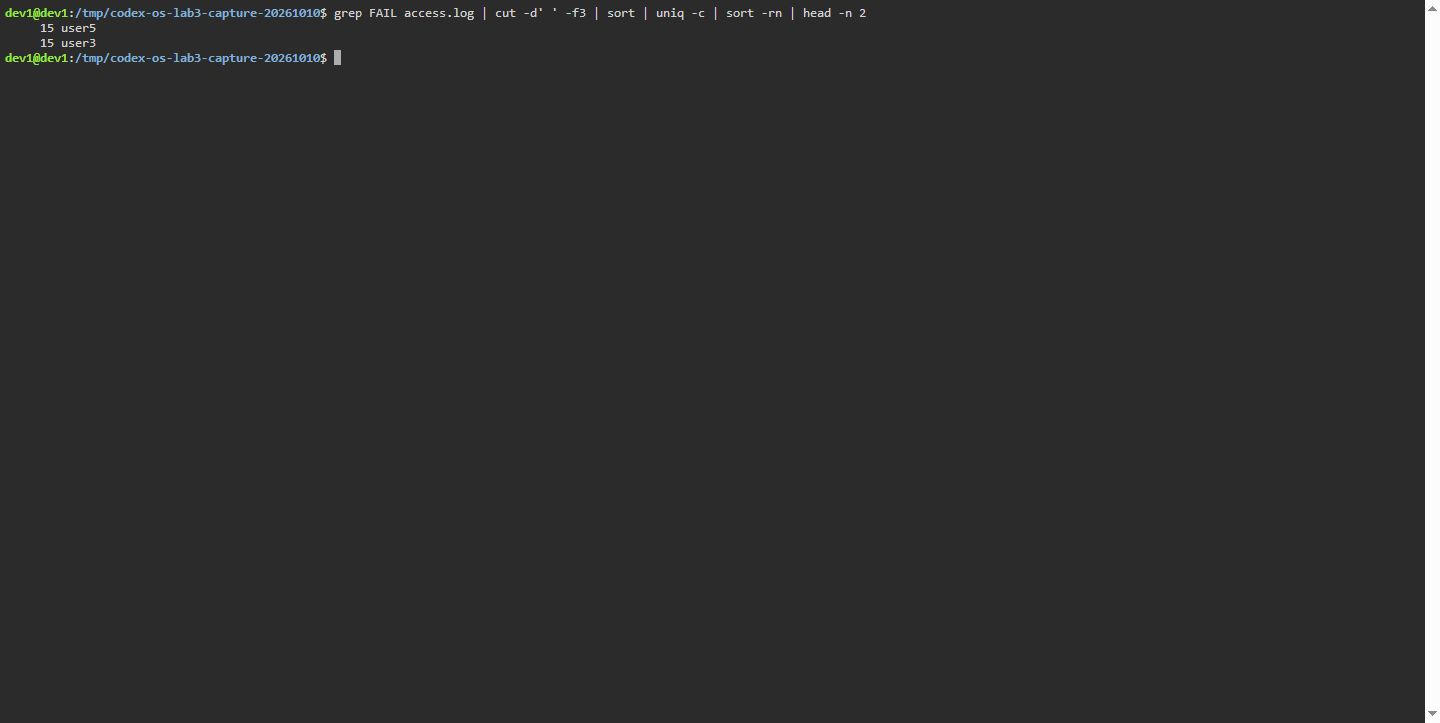
\includegraphics[width=0.88\textwidth]{figures/fig4_4_most_failures.jpg}
\caption{Terminal capture, Dev1 Debian GNU/Linux 13, 10 October 2026: Users exhibiting the greatest failure frequency.}
\label{fig:q4}
\end{figure}

\subsection{Q5: Activity breakdown for user3}
\begin{verbatim}
echo "user3 total: $(grep -c 'user3 ' access.log), \
failed: $(grep 'user3 ' access.log | grep -c FAIL)"
\end{verbatim}
The 9 October Debian 13 log records 72 total requests by \texttt{user3}, of which 15 failed (Figure \ref{fig:q5}).

\begin{figure}[H]
\centering
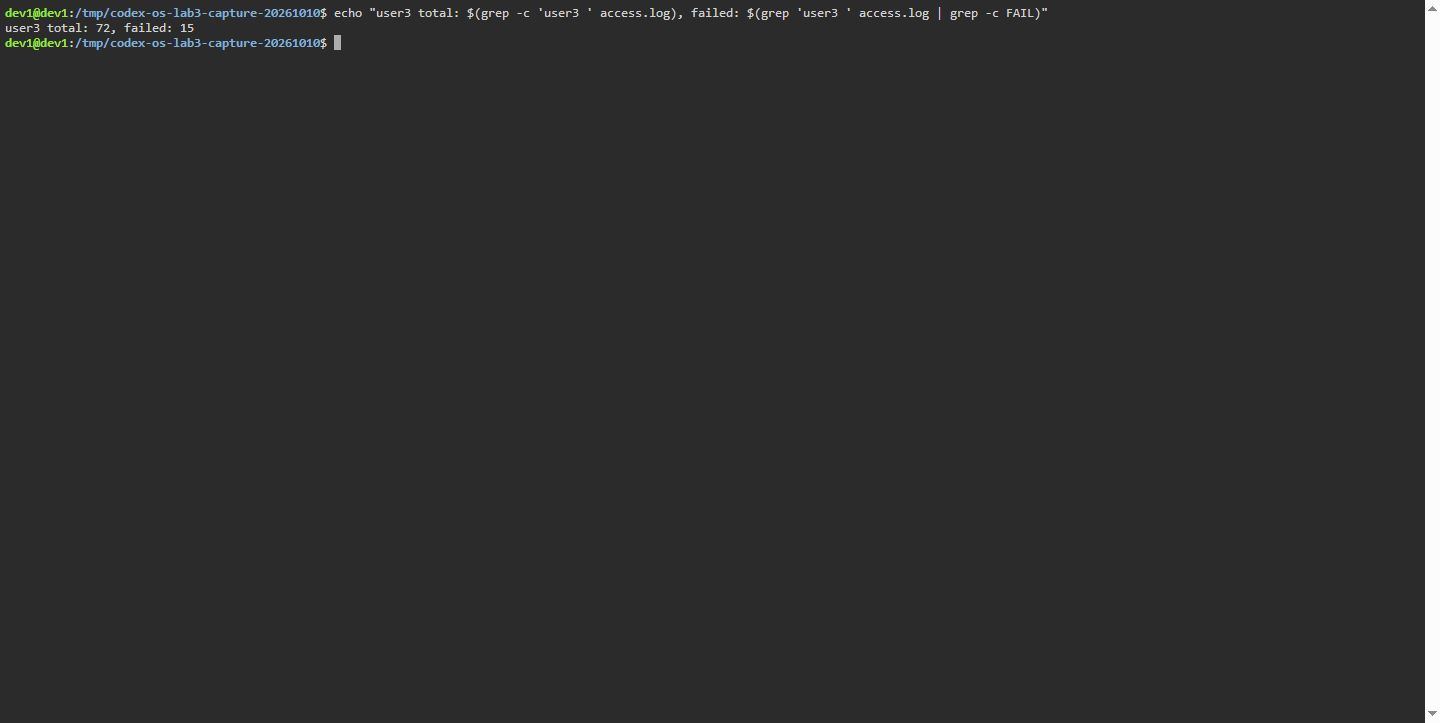
\includegraphics[width=0.88\textwidth]{figures/fig4_5_user3_counts.jpg}
\caption{Terminal capture, Dev1 Debian GNU/Linux 13, 10 October 2026: user3 request count and failed requests.}
\label{fig:q5}
\end{figure}

\subsection{Q6: Last three failed requests}
\begin{verbatim}
grep FAIL access.log | tail -n 3 | cut -d' ' -f2,3
\end{verbatim}
The 9 October Debian 13 log records \texttt{10:10 user0}, \texttt{10:15 user5}, and \texttt{10:20 user3} as the last three failed rows (Figure \ref{fig:q6}).

\begin{figure}[H]
\centering
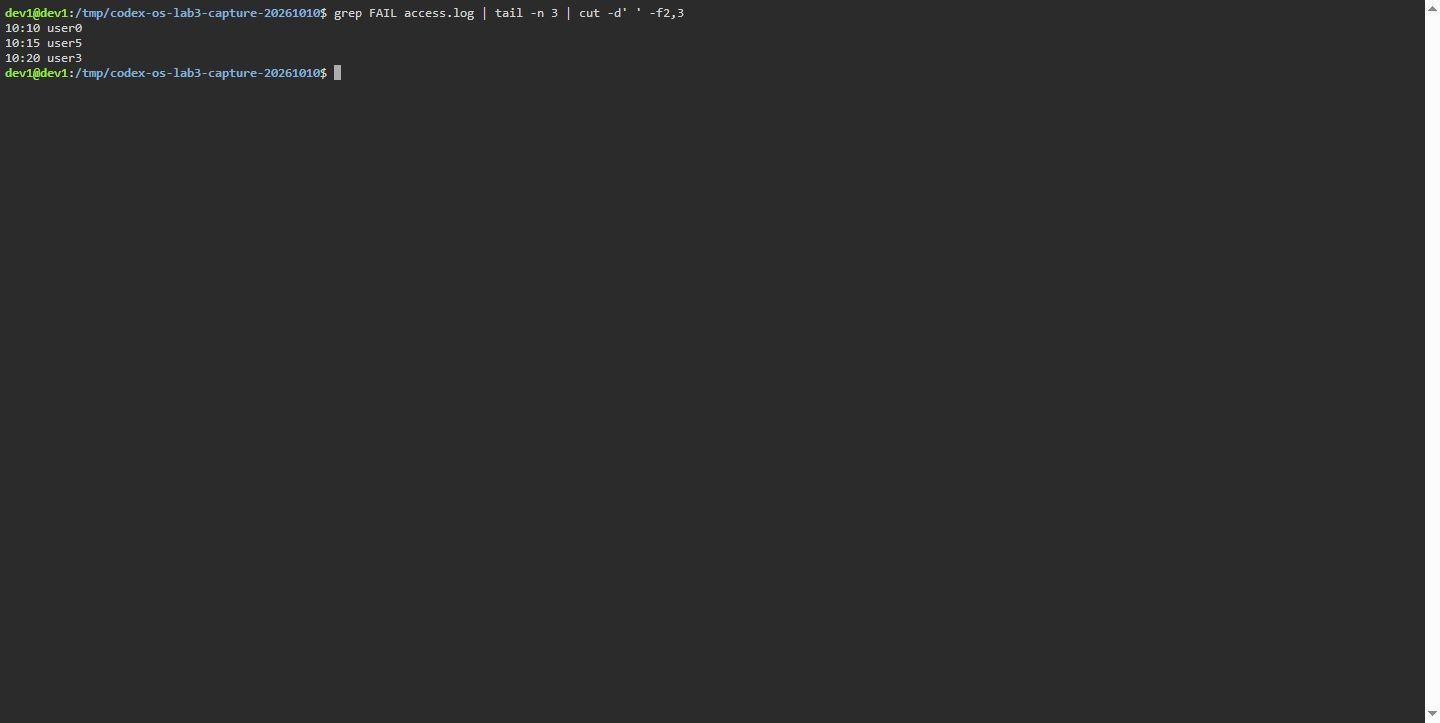
\includegraphics[width=0.88\textwidth]{figures/fig4_6_last3_failures.jpg}
\caption{Terminal capture, Dev1 Debian GNU/Linux 13, 10 October 2026: last three failed request rows.}
\label{fig:q6}
\end{figure}

\subsection{Q7: Accounts per login shell in /etc/passwd}
\begin{verbatim}
cut -d: -f7 /etc/passwd | sort | uniq -c | sort -rn
\end{verbatim}
The 10 October terminal capture records 29 \texttt{/usr/sbin/nologin}, 3 \texttt{/bin/false}, 2 \texttt{/bin/bash}, and 1 \texttt{/bin/sync}. These counts depend on the host.

\begin{figure}[H]
\centering
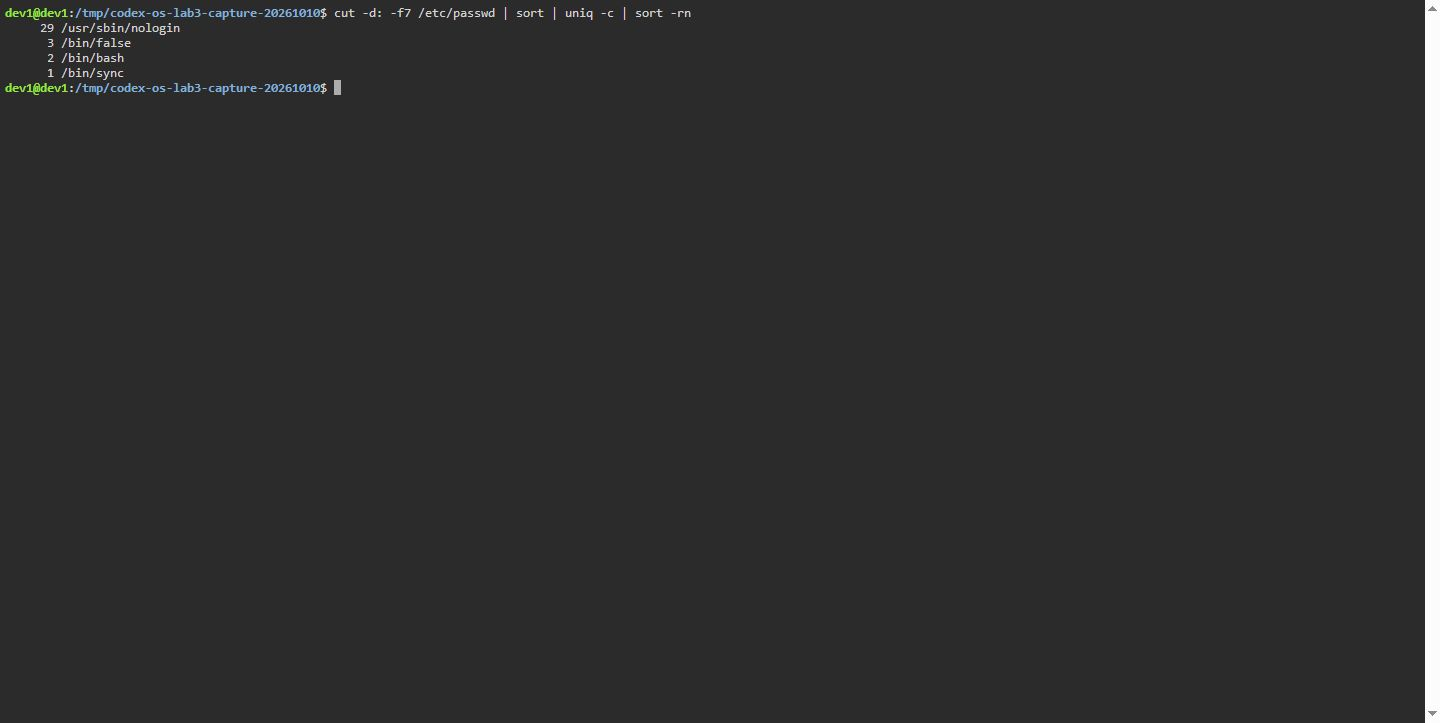
\includegraphics[width=0.88\textwidth]{figures/fig4_7_login_shells.jpg}
\caption{Terminal capture, Dev1 Debian GNU/Linux 13, 10 October 2026: account counts by login shell.}
\label{fig:q7}
\end{figure}



\subsection{Q8: Line count discrepancy between ls and ls -l}
\begin{verbatim}
ls /etc | wc -l ; ls -l /etc | wc -l
\end{verbatim}
The 10 October terminal capture records 196 lines for \texttt{ls /etc | wc -l} and 197 for \texttt{ls -l /etc | wc -l}; the one-line difference is the \texttt{total} summary line in long format.

\begin{figure}[H]
\centering
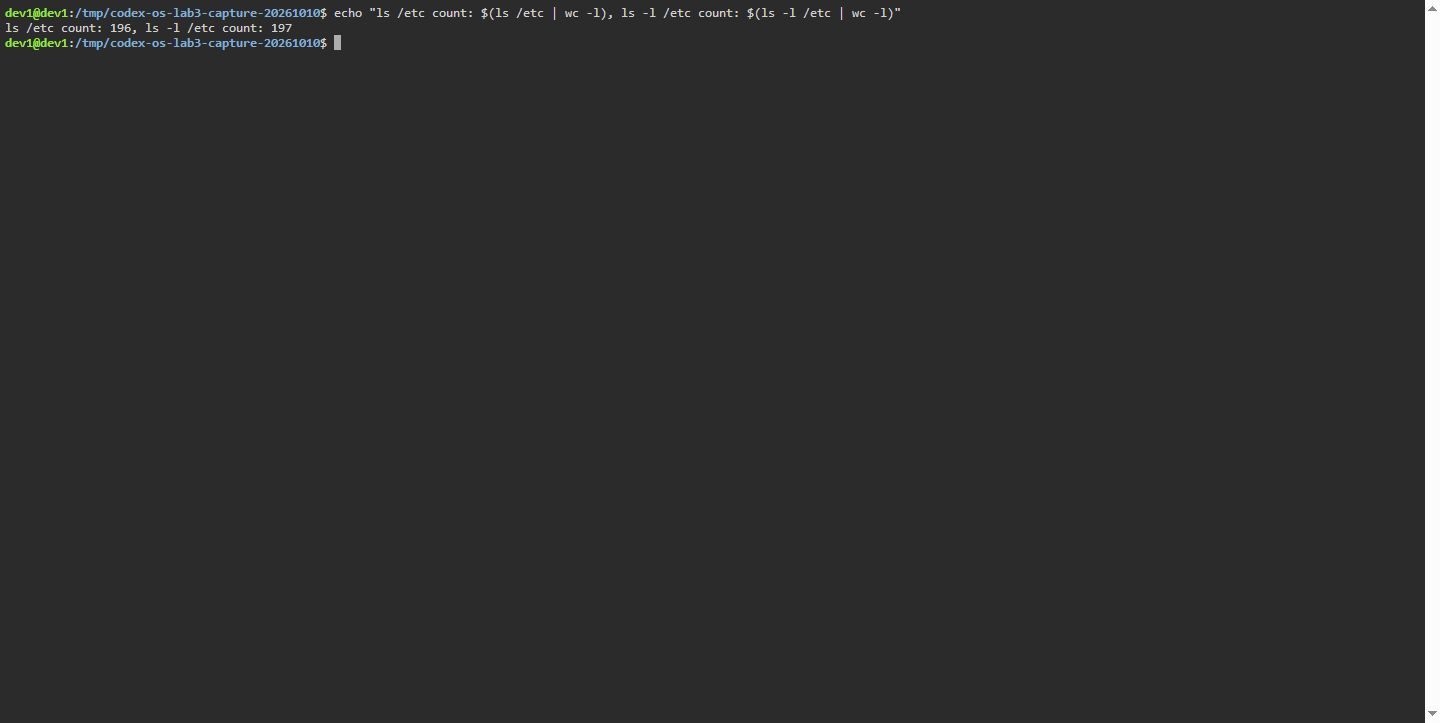
\includegraphics[width=0.88\textwidth]{figures/fig4_8_ls_wc_diff.jpg}
\caption{Terminal capture, Dev1 Debian GNU/Linux 13, 10 October 2026: line counts with and without long listing format.}
\label{fig:q8}
\end{figure}



\subsection{Full pipeline suite execution and bonus}
All one-liner queries were bundled in \texttt{oneliners.sh}. The bonus regex query:
\begin{verbatim}
grep -E '10:[0-5]0 .* FAIL' access.log
\end{verbatim}
isolates requests occurring at 10-minute intervals that failed, yielding exactly 50 matching lines (Figure \ref{fig:q9}).

\begin{figure}[H]
\centering
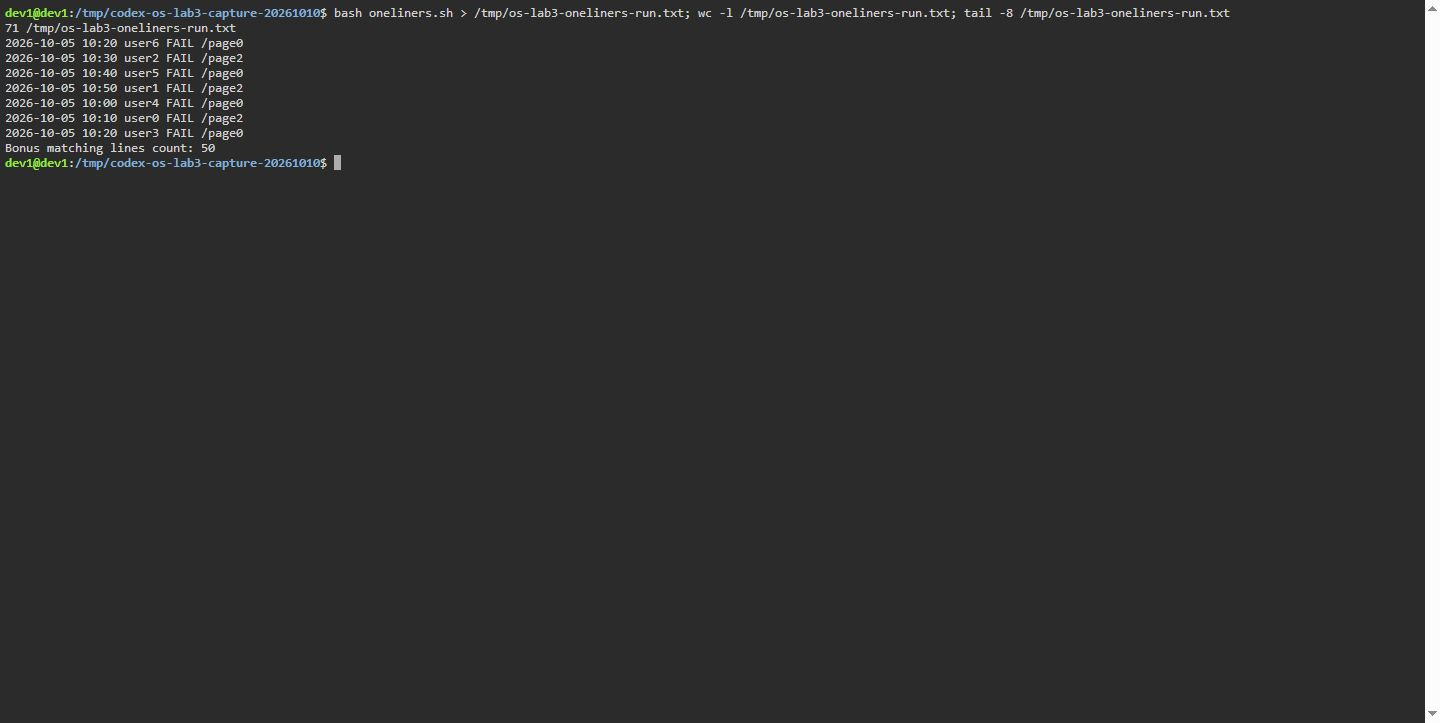
\includegraphics[width=0.88\textwidth]{figures/fig4_9_oneliners_run.jpg}
\caption{Terminal capture, Dev1 Debian GNU/Linux 13, 10 October 2026: complete one-liner run and bonus match count.}
\label{fig:q9}
\end{figure}

\chapter{Structured Shell Automation}

\section{Implementation of report.sh}
The analytical one-liners were integrated into an executable automation script \texttt{report.sh}. The script incorporates argument verification, exit code signaling, and dynamic looping over users \texttt{user0} through \texttt{user6} (Figure \ref{fig:script_src}).

\begin{figure}[H]
\centering
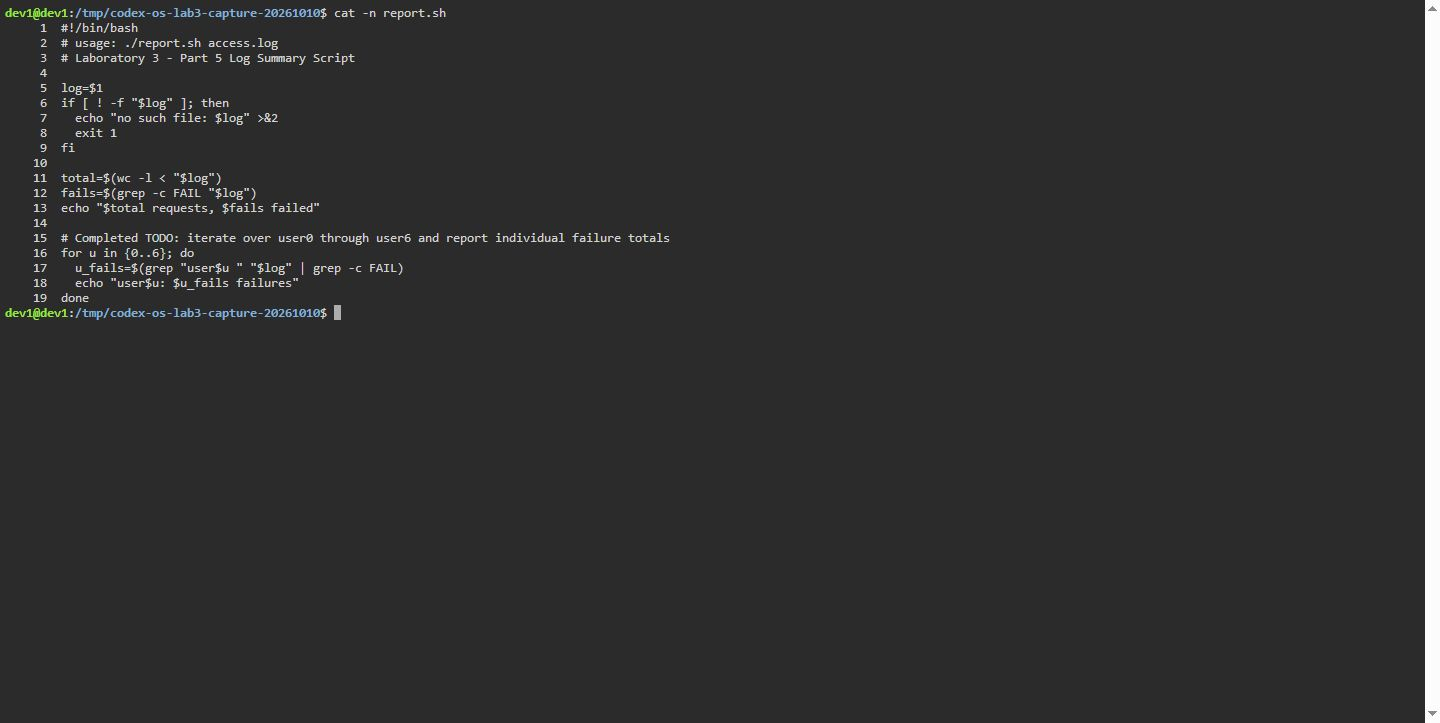
\includegraphics[width=0.88\textwidth]{figures/fig5_1_report_script.jpg}
\caption{Terminal capture, Dev1 Debian GNU/Linux 13, 10 October 2026: Source implementation of report.sh with completed user iteration.}
\label{fig:script_src}
\end{figure}

Execution against \texttt{access.log} correctly parses the 500 lines and outputs individual user failure metrics (Figure \ref{fig:running_report}).

\begin{figure}[H]
\centering
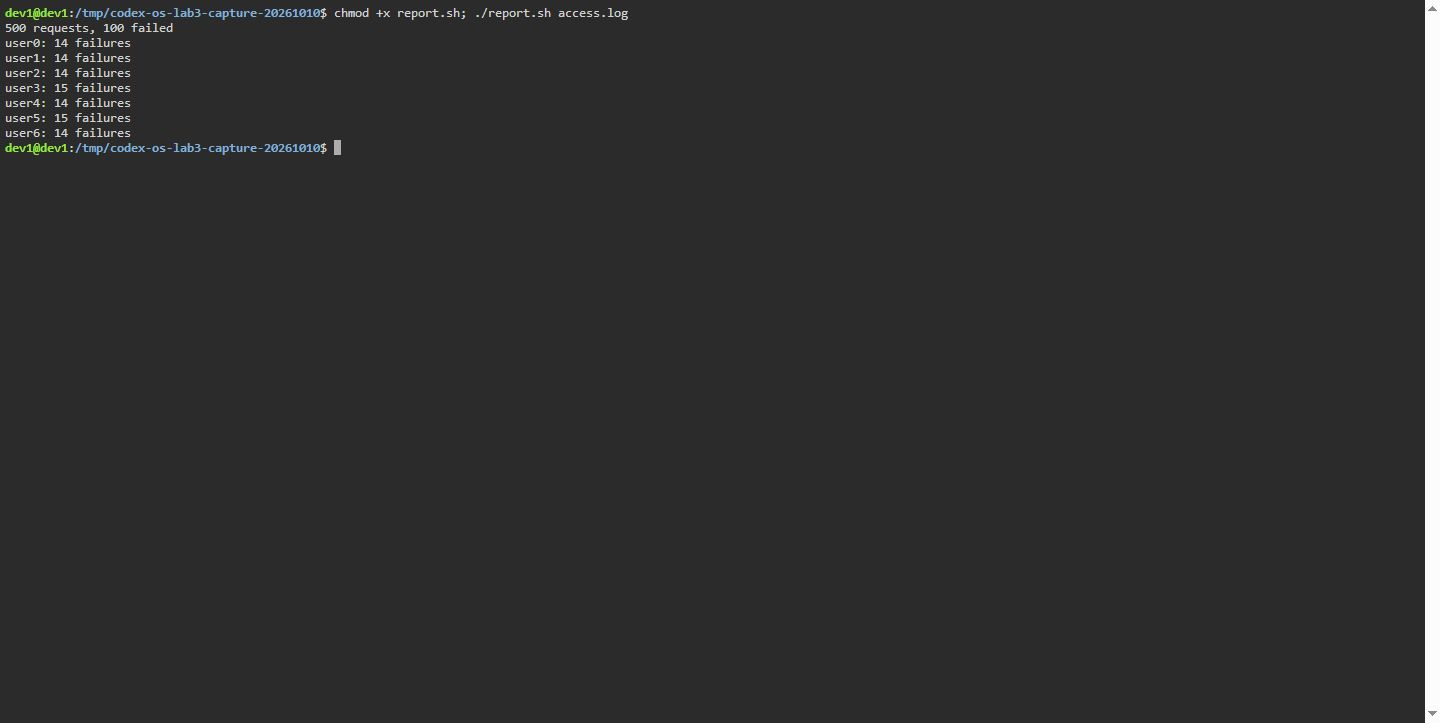
\includegraphics[width=0.88\textwidth]{figures/fig5_2_running_report.jpg}
\caption{Terminal capture, Dev1 Debian GNU/Linux 13, 10 October 2026: Execution of report.sh against the generated access dataset.}
\label{fig:running_report}
\end{figure}

When supplied an invalid or missing file, the script writes diagnostic messages to stderr and terminates with status 1 (Figure \ref{fig:missing_error}).

\begin{figure}[H]
\centering
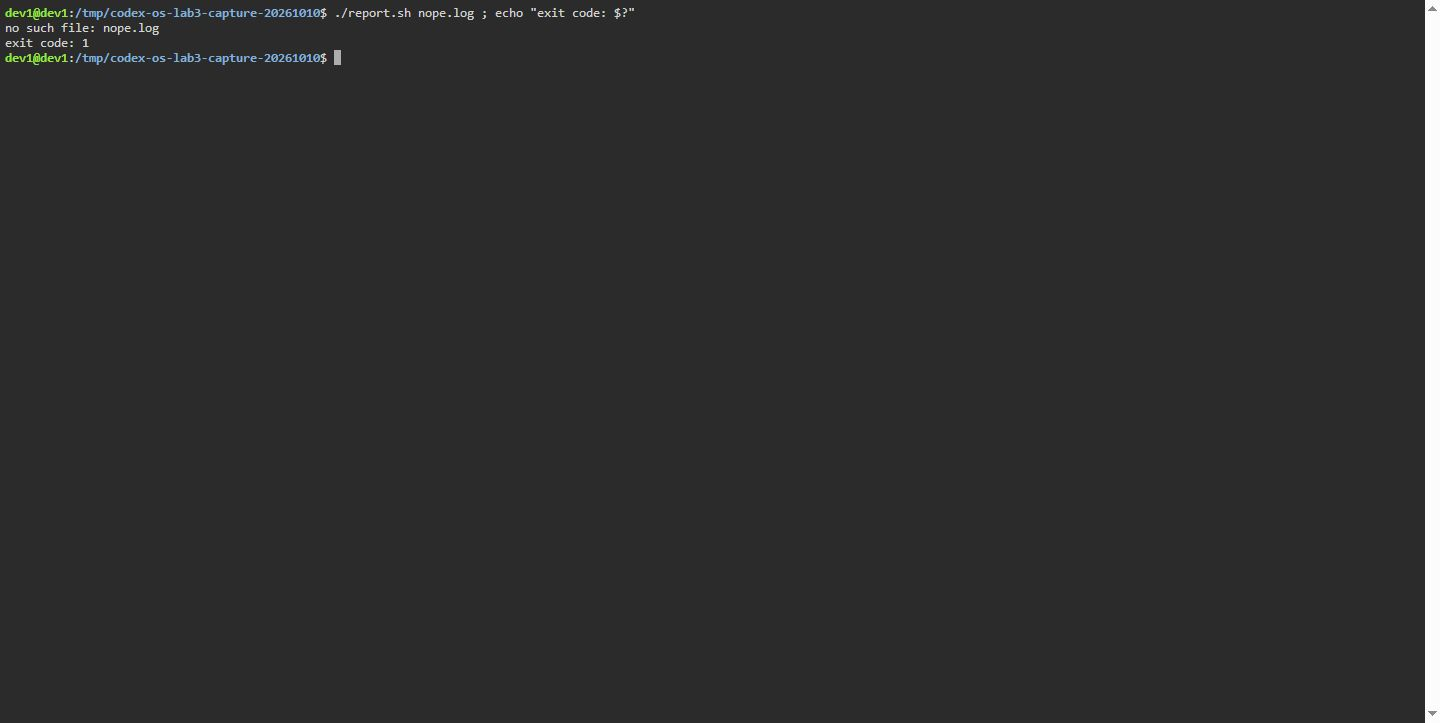
\includegraphics[width=0.88\textwidth]{figures/fig5_3_missing_file_error.jpg}
\caption{Terminal capture, Dev1 Debian GNU/Linux 13, 10 October 2026: Diagnostic error reporting and non-zero exit code.}
\label{fig:missing_error}
\end{figure}

\section{Cron daemon integration}
The optional cron task ran on Dev1 Debian GNU/Linux 13 using a temporary copy of the Lab 3 files. Cron was active and the user crontab was empty before the test. The following one-minute entry ran \texttt{report.sh} against the copied dataset and appended its output to \texttt{report.log}:

\begin{lstlisting}
* * * * * /tmp/codex-os-lab3-4-20261009/lab3/report.sh /tmp/codex-os-lab3-4-20261009/lab3/access.log >> /tmp/codex-os-lab3-4-20261009/lab3/report.log 2>&1
\end{lstlisting}

The log recorded four complete runs during the approximately two-minute check. Its complete contents were:

\begin{lstlisting}
500 requests, 100 failed
user0: 14 failures
user1: 14 failures
user2: 14 failures
user3: 15 failures
user4: 14 failures
user5: 15 failures
user6: 14 failures
500 requests, 100 failed
user0: 14 failures
user1: 14 failures
user2: 14 failures
user3: 15 failures
user4: 14 failures
user5: 15 failures
user6: 14 failures
500 requests, 100 failed
user0: 14 failures
user1: 14 failures
user2: 14 failures
user3: 15 failures
user4: 14 failures
user5: 15 failures
user6: 14 failures
500 requests, 100 failed
user0: 14 failures
user1: 14 failures
user2: 14 failures
user3: 15 failures
user4: 14 failures
user5: 15 failures
user6: 14 failures
\end{lstlisting}

The temporary cron entry was removed, and the user crontab was empty afterward. The log records a run on the remote Dev1 host; it does not establish use of the assigned course laptop or VM.

\section{Answers to Part 5 Observe questions}
\begin{utmenumerate}
\item \textbf{What does the first line \texttt{\#!/bin/bash} do, and what happens if you run \texttt{./report.sh} before \texttt{chmod +x}?} \\
The shebang line \texttt{\#!/bin/bash} informs the kernel's \texttt{execve()} system call which interpreter binary to load when executing the script. Attempting to run \texttt{./report.sh} without execute permissions returns \texttt{bash: ./report.sh: Permission denied}.
\item \textbf{Why must you type \texttt{./report.sh} and not just \texttt{report.sh}?} \\
The shell only traverses directories explicitly listed in \texttt{\$PATH}. The current working directory (\texttt{.}) is omitted from \texttt{PATH} by default to prevent accidental execution of untrusted local binaries. Prefacing with \texttt{./} provides an explicit relative path.
\item \textbf{Why does the script write the error with \texttt{>\&2} and end with \texttt{exit 1}?} \\
\texttt{>\&2} redirects error strings to standard error (descriptor 2), preserving standard output for clean pipeline data. \texttt{exit 1} signals abnormal termination to calling environments and conditional operators.
\end{utmenumerate}

\utmconclusions
The terminal figures show actual command output captured on the Dev1 Debian GNU/Linux 13 host. The handout calls for a Linux laptop or VM; this report does not establish which assigned environment was used.

\begin{thebibliography}{9}
\bibitem{nemeth} Nemeth, E., Snyder, G., Hein, T. R., Whaley, B., \& Mackin, D. (2017). \textit{UNIX and Linux System Administration Handbook} (5th ed.). Addison-Wesley Professional.
\bibitem{shotts} Shotts, W. (2019). \textit{The Linux Command Line: A Complete Introduction} (2nd ed.). No Starch Press.
\bibitem{posix} IEEE \& The Open Group. (2018). \textit{The Open Group Base Specifications Issue 7 / IEEE Std 1003.1-2017 (POSIX.1)}. Shell Command Language.
\bibitem{bash} Free Software Foundation. (2024). \textit{Bash Reference Manual}. Version 5.2.
\end{thebibliography}

\end{document}
